\documentclass[11pt]{article}
\usepackage[margin=0.85in]{geometry}
\usepackage{amsmath,amssymb,graphicx,hyperref}
\setlength{\parindent}{0pt}\setlength{\parskip}{6pt}
\setlength{\emergencystretch}{3em}
\begin{document}
{\Large Exact nonconstant lower-chart control from two lines}\\
November 13, 2026. Unsigned producer evidence [pcc:unverified].

\textbf{Inputs and construction.} Over $\mathbb F_{17}$ reuse
$f=X^3+2X+2$. Choose $L=2X+8$, $M=4X+6$. Lean checks
\[
 A=f+LM=X^3+8X^2+12X+16,\quad B=L+M=6X+14=6H,\ H=X+8.
\]
The universal commutative-ring two-line identity and its exact specialization give
\[
\begin{split}
 (f+LM)^2-f(L+M)^2&=(f-L^2)(f-M^2),\\
 A^2-fB^2&=(X-5)(X-6)(X-10)X(X-3)(X-13)=G.
\end{split}
\]
All six nodes are distinct, and each supplied point
$(5,1),(6,3),(10,11),(0,6),(3,1),(13,7)$ satisfies the cubic equation.
At target $Q=(0,6)$, $A(0)-6B(0)=0$ and $A(0)\ne0$.

\textbf{Explicit quotient data.} Let $F=A$ and
\[
 U=16X^3+11X^2+6X+12,\qquad V=X^2+6X+4.
\]
The actual identity $UF+V(fH)=1$ is checked. Degrees and monicity give the
full chart $a=3,b=1,d=6$, with $B$ genuinely nonconstant.
For $\mu(P)=[X^2]((PV)\bmod F)$, the supplied norm equation derives
$\mu(G)=0$. All hypotheses of the actual canonical matrix-pencil theorem are
instantiated; the coordinate dimension is6.

\begin{center}
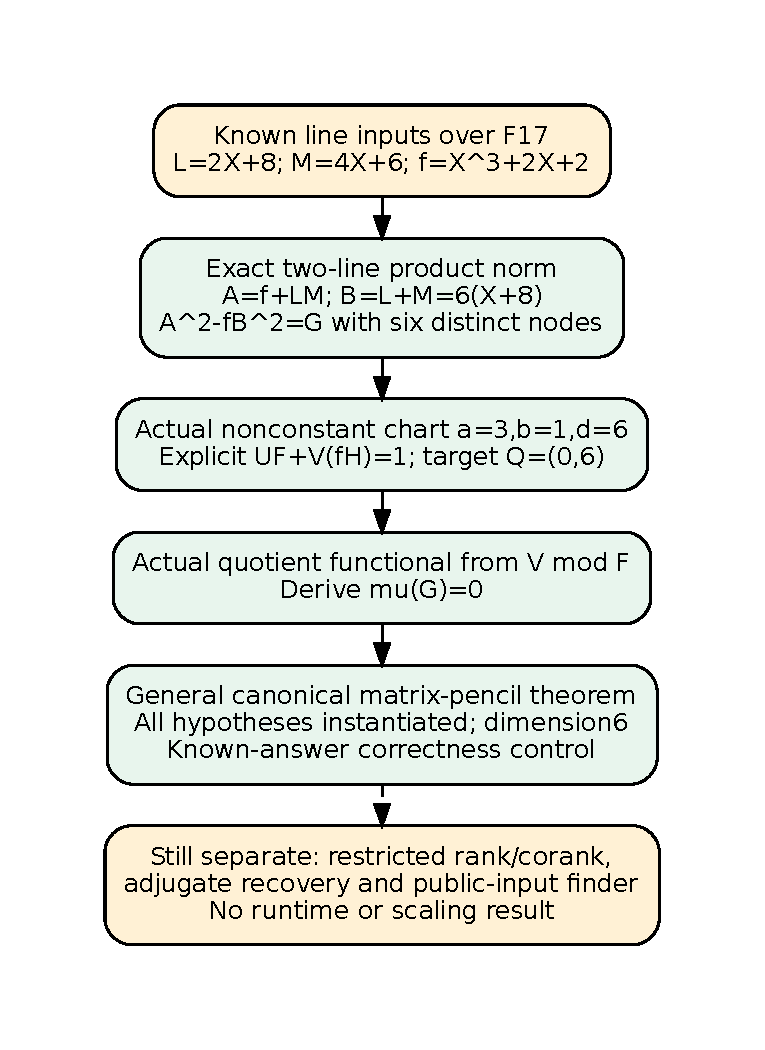
\includegraphics[width=0.9\linewidth,height=0.36\textheight,keepaspectratio]{control.pdf}
\end{center}

\newpage
{\Large Control scope, exact checks and next validation}

\textbf{Why this control.} The earlier constant-$B$ fixture did not exercise
a positive-degree quotient modulo $H$. This algebraically constructed
nonconstant chart covers that mechanism with supplied norm, inverse and branch
data. It is a known-answer correctness control, with no random search or
host-dependent runtime measurement. Exact equalities are independent of CPU
contention. Restricted rank/corank, adjugate recovery and search complexity
are not established by the current control.
The supports are constructed with the witness; relation finding over an
independently generated known-label online factor base is not tested.

\textbf{Source and map.} Module: \path{NormNonconstantControl.lean}.

Frozen source \path{cbfdaad42}. The map covers universal two-line norm;
exact construction, cubic factors and prescribed norm; lower scaling and
B\'ezout; branch/nonzero conditions; monicity/degrees; node distinctness and
curve points; quotient target annihilation; coordinate dimension; and
canonical matrix-pencil instantiation. Full declaration names are in the
Markdown map. Twenty-two scoped interpretive records bind the
reported declarations; all standing remains unsigned. The older NormRank
source supplies the previous curve's nonsingularity and point-count checks.

\textbf{Checks and failures.} Lean4.35.0, unchanged pinned dependencies.
Build004 passes3150 jobs without new-source warnings. Full tracked-source
audit covers143 declarations, zero failing and zero additional trusted axioms.
Separate fresh import-inclusive replay exits0; its completion receipt is retained.
Only \path{propext}, \path{Classical.choice}, \path{Quot.sound} are admitted.
Build001 left arithmetic side goals and dependent-index rewrite issues;
actual degree-indexed families with a separate dimension proof resolve them.
Build002 left nonzero6 over F17, discharged by kernel decide. Build003 passed;
build004 removes unused new tactics. All logs are retained. No signed PCC
verdict or kernel bypass is claimed.

\textbf{Native identity.} \path{IDC1h36c0f0c618539c35} checks universal
\path{twoLineNorm} at32 statement-derived and32 extra-stream points through
the unchanged maintained checker. The exact source pointer is to a universal
CommRing theorem, not a finite-field-only equality. It does not execute Lean
or establish finite-field/matrix/search claims. Its adapter's22 inherited
tests pass, including tamper/statement-swapping controls. No timing claim.

\textbf{Next.} Actual arbitrary-pair bilinear/branch transfer, coordinate
injectivity and corank; then guarded adjugate recovery and an explicit
restricted control. Exceptional charts and a public-input moment finder with
accounted $2^{o(n)}$ bit cost remain separate. Current data uses a supplied
witness. Reachability through $W_{\rm base}+C(T)H(T)$ also remains open.

\textbf{Sources and resources.} Proposed two-line control, existing exact
F17 fixture, actual matrix/functional source, pinned degree/monicity APIs.
KB/conductor unavailable; bounded fallback, no priority claim for elementary
line norms. No paid job, runtime/scaling campaign or budget override; monthly
isolab budget exhausted. No benchmark/leaderboard/ecdb changes. Source-linked
Markdown, editable DOT/SVG, diagram/report PDFs and raw evidence accompany this
known-answer result.
\end{document}
